% !Mode:: "TeX:UTF-8"
% Author: Zhengxi Tian
% Email: zhengxi.tian@hotmail.com

\chapter{相关工作}\label{ch:related_work}
% ------------------ Models ------------------ %
\section{生成式模型}\label{sec:generative_model}
一个生成式模型定义了给定输入序列$X = x_1, x_2, \cdots, x_n$,
任意输出序列$Y = y_1, y_2, \cdots, y_m$的条件概率:
\begin{align}
    p(Y|X) = P(y_1, y_2, \cdots, y_m|x_1, x_2, \cdots, x_n)
    \label{eqn:generative_conditional_probability}
\end{align}
模型的训练目标就是在数据集$S$上最大化给定$X$,$Y$的对数概率(Log Probability):
\begin{align}
    \mathit{L} = \frac{1}{|S|} \sum_{(Y, X) \in S} \log p(Y|X)
\end{align}
从这个角度来看,语言模型\upcite{NNLM,RNNLM}(Language Model)和编解码器(Encoder-Decoder)都属于生成式模型,
因为它们都定义了条件概率$p(Y|X)$。
生成式模型把一个长度可变的序列$X$映射到另一个长度可变的序列$Y$,且$X$和$Y$的长度可以不相等。
循环神经网络(RNN)为这个问题提供了自然的解决方案。
% RNN
RNN的基本思想是:序列由有序的元素组成,每一个时刻(Time Step)输入并输出一个元素,同时更新内部的隐层状态(Hidden State)。
在时间轴上展开的RNN和一般的前馈神经网络(Feed Forward Neural Networks)很像,不过每一个时刻的权重矩阵都是共享的。
这个共享的权重矩阵$A$又被称为循环矩阵(Recurrent Matrix)。
循环矩阵的作用是保存输入序列的顺序信息,并把当前时刻的输入序列编码成一个定长向量。
图~\ref{fig:RNN_unrolled}\footnote{http://colah.github.io/posts/2015-08-Understanding-LSTMs/}
描绘了简化的RNN结构。
\begin{figure}[H]
    \centering
    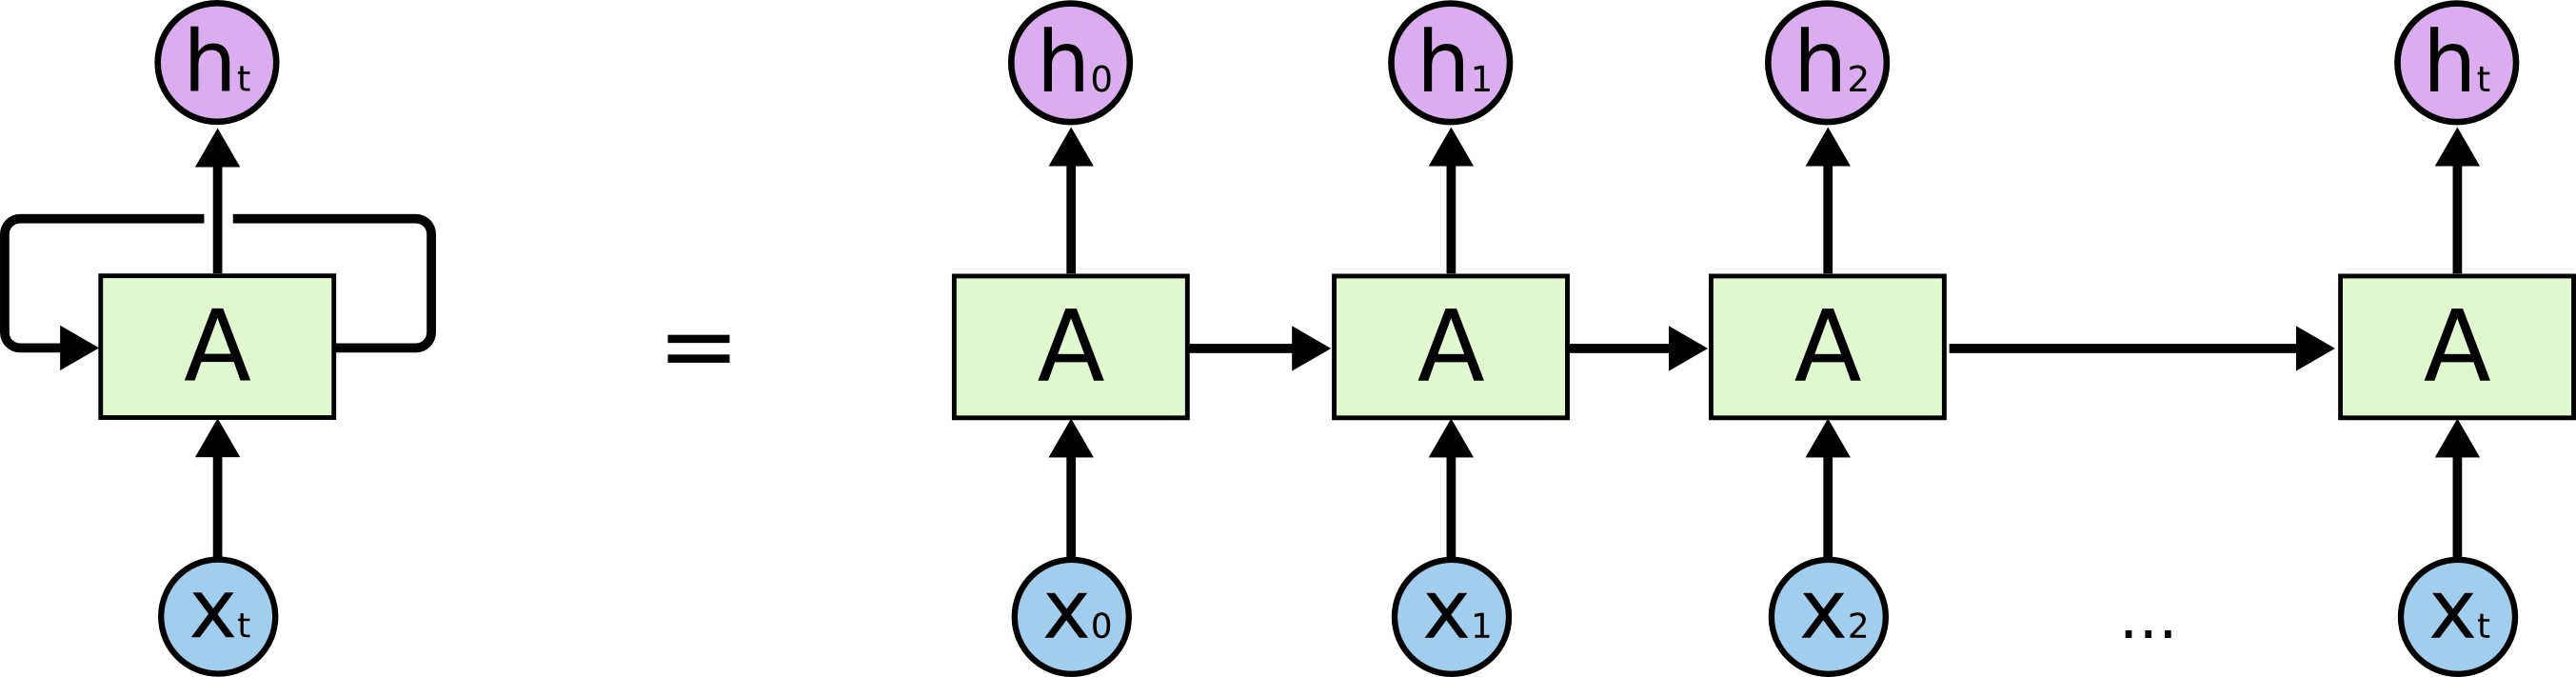
\includegraphics[width=0.6\textwidth]{figure/RNN-unrolled.png}
    \caption{RNN的一般表示和展开表示}
    \label{fig:RNN_unrolled}
\end{figure}

% ------------------ RNN types ------------------ %
根据是否使用了某种门单元,RNN可分为普通RNN\upcite{RNNLM},
LSTM\upcite{LSTM}和GRU\upcite{GRU}。
根据是否对反向序列(Reversed Sequence)建模,RNN可分为单向RNN(Unidirectional RNN)
和双向RNN(Bidirectional RNN)\upcite{BiRNN}。
由于普通RNN受到梯度消失的影响,目前学界普遍采用LSTM或者GRU;
尽管后者受到梯度爆炸的影响,但是可以通过梯度剪裁(Gradient~Clipping)
\upcite{GoogleChatbot}解决。
采用多层RNN组成的深度神经网络比单层RNN能获得更好的性能\upcite{GoogleChatbot}。

\subsection{RNN语言模型}\label{subsec:RNNLM}
% ---------------- RNNLM ------------------ %
RNN语言模型可以给出序列$X=x_1, x_2, \cdots, x_n$的概率分布:
\begin{align}
    p(X) = \prod_{i=1}^{n} p(x_i|x_1, x_2, \cdots, x_{i-1})
    \label{eqn:language_model_probability}
\end{align}

RNN语言模型\footnote{为了简洁起见,我们描述了普通RNN。LSTM和GRU有着更复杂的数学表达式。}
通过神经网络中的参数来估计公式~\ref{eqn:language_model_probability}~乘积中的一项:
\begin{align}
    p(x_i = w|x_1, x_2, \cdots, x_{i-1}) = \frac{\exp{o_{tw}}}{\sum_{v=1}^V \exp{o_{tv}}}
    \label{eqn:language_model_estimation}
\end{align}
$o_t$是RNN的在$t$时刻的输出向量,$V$是词汇表的大小。
公式~\ref{eqn:language_model_estimation}~的右边本质上是对一个长度为$V$的向量进行softmax运算。
$t$时刻的输出向量是由输出矩阵$W_{out}$和$t$时刻隐层状态$h_i$相乘得到的:
\begin{align}
    o_i &= h_i^T W_{out}
\end{align}
而$h_i$则是当前输入$x_i$和上一时刻的隐层状态$h_{i-1}$在输入矩阵$W_{in}$和循环矩阵$W_{hh}$分别作用后再相加的结果:
\begin{align}
    h_i &= \sigma \left( x_i^T W_{in} + h_{i-1}^T W_{hh} \right)
\end{align}
RNN语言模型在训练时最大化训练集上的句子的对数概率:
\begin{align}
    \mathit{L(X)} = \sum_{i=1}^n \log p(x_i|x_1, x_2, \cdots, x_{i-1})
\end{align}
在预测时,对模型输入消息$m$,从模型的给出的概率分布中用某种搜索方法,如Beam Search可得出响应$r$。

\subsection{Seq2Seq框架}\label{subsec:Seq2Seq}
% ------------------ Seq2Seq ------------------ %
Seq2Seq框架使用两个拥有独立参数的RNN分别作为编码器和解码器。
尽管编解码器不一定都使用RNN\upcite{JointTransAlign},本文仅关注使用RNN的Seq2Seq变体。
首先,编码器把输入序列$X$编码成一个定长向量$v$。
该向量又称为思考向量(Though Vector),是编码器完全读取输入序列后的隐层状态(Last Hidden State)。
接着,解码器以$v$为初始隐层状态(Initial Hidden State),像一个RNN语言模型一样对输出序列进行预测。
整个过程可以描述为:编码器把输入序列$X$变换成某种压缩编码$v$,再由解码器把$v$还原为另一个序列$Y$,
Seq2Seq把公式~\ref{eqn:generative_conditional_probability}~
作了如下转化:
\begin{align}
    p(y_1, y_2, \cdots, y_m|x_1, x_2, \cdots, x_n) = \prod_{i=1}^m p(y_i|v, y_1, y_2, \cdots, y_{i-1})
\end{align}
其中$v$是以$f$为门单元的编码器的最后一个隐层状态:
\begin{align}
    h_i &= f(x_i ,h_{i-1}) \\
    c &= h_n
\end{align}
编码器和解码器以同一个目标函数同时训练。
为了更好的处理长序列,Seq2Seq一般引入注意力机制(Attention Mechanism)
\upcite{
JointTransAlign,
EffectiveAttention},使输入序列的信息不必全部通过固定长度的向量$v$传递。
解码器能自动关注和当前输出最相关的输入部分,实现输入序列与输出序列的对自动对齐(Alignment)。
注意力机制使传统Seq2Seq模型对较长输入也具有鲁棒性。

\subsection{解码算法}\label{subsec:decode}
% ------------------ Decoding ------------------ %
生成式模型仅仅定义了条件概率$p(Y|X)$,在推理阶段(Inference),需要采用某种启发式搜索算法从概率分布中
生成输出$Y$,这个过程又称为解码(Decode)。
最简单的搜索算法是贪心搜索(Greedy Search):在每一时刻都输出条件概率最大的单词:
\begin{align}
    y_i = \argmax p(y_i|y_1, y_2, \cdots, y_{i-1}, X)
\end{align}
因为各个$y_i$的概率都不是独立的,而是受之前输出的单词的影响,贪心搜索不能保证得到概率最大的输出序列。
随机取样(Random Sampling)在每一时刻都从模型生成的全体词汇的概率分布中随机选取一个单词。
这样就使输出就带有不确定性,在一定程度上增加了输出的多样性。
Serban等人曾发现随机取样的输出能避免单调响应的问题,并且能产生多样化的,
话题相关的输出\upcite{HRED}。
最为常用的方法是集束搜索(Beam Search),它在生成整个句子的过程中维护一个大小为$B$的列表,称为集束(Beam)。
算法开始时,集束初始化为模型生成的$B$个概率最高的单词。
在每一个时刻开始时,集束中都有$B$个部分生成的句子,它们称为候选$Y_c$。
在每一个时刻,算法对集束中的每一个候选都生成$B$个概率最大的下一个单词$w_{i+1, c}$,从而形成$B \times B$个部分生成的句子$Y_{ex}$,
称为扩展的候选集。从扩展的候选集中,只保留前$B$个概率$p(Y_{ex}|X)$最大的句子。
算法不断迭代直到在某次对候选集的扩展中,某些候选中产生了句子结束符号(End-of-Sentence,EOS),
于是概率最大而且完成了的候选句子将作为输出。

% ------ Diverse Beam, MMI, Stochastic Greedy Sampling ------ %
为了增加模型输出的多样性,学者们提出了许多改进的解码算法。
Li等人在\cite{DiverseBeam}中提出在标准集束搜索中,对来自相同父节点的候选加以惩罚,即鼓励来自不同父节点的候选。
他们在\cite{MMI}中提出用最大互信息(MMI)对标准集束搜索生成的候选列表进行重新排序,
从而提高候选输出的反向概率(Backward Probability),
即给定输出$Y$,输入$X$的条件概率$p(Y|X)$,使输出对输入更有针对性。
他们在\cite{Distill}中提出了一种名为随机贪心取样(Stochastic Greedy Sampling)的解码算法,
以求在随机取样和贪心搜索之间找到一个平衡点。与传统的随机取样不同,他们的算法只在条件概率最高的前$K$个候选单词中取样,
参数$K$控制了随机取样和贪心搜索之间的比例:$K$越大,算法越接近随机取样,$K$越小,算法越接近贪心搜索。
这些改进的解码算法在不同程度上提高了响应的多样性。

% ------------------ Metrics ------------------ %
\section{自动化评价指标}\label{sec:automatic_metric}
\subsection{评价指标简介}\label{subsec:metrics_intro}
机器翻译领域已有大量和人类评价相关性较高的指标,例如
BLEU\upcite{BLEU},
NIST\upcite{NIST},
METEOR\upcite{METEOR},
BEER\upcite{beer},
CHRF\upcite{chrf},
TER\upcite{HTER}等等。
然而,适用于开放领域的,面向闲聊的对话系统的指标要少得多;
在考察本领域对自动指标的使用情况之前,先对各种指标作一个简要介绍。

% --------------- BLEU ------------------ %
BLEU,Bilingual Evaluation Understudy\upcite{BLEU}是Papineni在2002年提出的,
用于机器翻译的自动评价指标。它是一个系统层面的评价指标,即评价一个系统在整个测试集上的性能。
BLEU指标只有一个参数$N$,表示要计算的各阶n-gram准确率的最大值;例如$N = 4$表示要计算1-gram到4-gram的准确率。
准确率指的是系统输出和参考输出之间的n-gram重叠数占系统输出总的n-gram的比例。
BLEU由在整个数据集上计算的各阶n-gram准确率的几何平均值(Geometric Mean)和简短惩罚系数(Brevity Penalty)相乘得到。
引入简短惩罚系数的原因是,较短的系统输出句子的准确率较高,需要矫正。
n-gram准确率的计算公式为:
\begin{align}
    p_n = \frac{
    \sum_{\mathcal{C} \in \{\textit{Candidates}\}
    \sum_{\textit{n-gram} \in \mathcal{C}}}
    \textit{Count}_{\textit{clip}}(\textit{n-gram})
    }{
    \sum_{\mathcal{C'} \in \{\textit{Candidates}\}}
    \sum_{\textit{n-gram}' \in \mathcal{C'}}
    \textit{Count}(\textit{n-gram}')
    }
\end{align}
Candidates为系统输出的句子集合,$\textit{Count}_{\textit{clip}}(\textit{n-gram})$为截断的n-gram共现数,
$\textit{Count}(\textit{n-gram}')$是Candidates中的总n-gram数。
简短惩罚系数BP的计算公式为
\begin{align}
    \textit{BP} =
    \begin{cases}
        \ 1 \ & \text{if} \  c > r \\
        \ e^{1 - r/c} \ & \text{if} \  c \leq r \\
    \end{cases}
\end{align}
其中$c$是模型输出句子的长度,$r$是参考输出句子的长度。
BLEU的最终公式为:
\begin{align}
    \textit{BLEU} = \textit{BP} \cdot \exp \left( \sum_{n=1}^N w_n \log p_n \right)
\end{align}
实际使用中一般取$N = 4$,$w_n = 1 / N$。
原始的BLEU容易在句子层面给出0分,人们提出了各种平滑处理\upcite{sBLEU-Smooth}。
本文在使用BLEU时也采用了一种平滑处理。

% ------------ ROUGE -------------- %
ROUGE,Recall-Oriented Understudy for Gisting Evaluation\upcite{ROUGE}是一种基于召回率的自动摘要领域的指标。
它有多个变体:ROUGE-N,ROUGE-L,ROUGE-W,ROUGE-S,以及ROUGE-SU,
分别使用了不同的计数单元(Counting Unit),如n-gram共现数、最长公共子序列(Longest Common Subsequence,LCS)和二元跳词(Skip-Bigram)等等。
这些指标的基础是信息检索领域常用的F-measure,即准确率$P$和召回率$R$的加权调和平均值:
\begin{align}
    \textit{F-measure} = \frac{(1 + \beta^2) RP}{R + \beta^2 P}
\end{align}
$\beta$控制准确率和召回率的相对重要性。
以下无特殊说明时,当指标是句子层面的时候,$n$是系统输出的句子的长度,$m$是参考输出的句子的长度;
当指标是摘要层面的时候,$n$是系统输出的摘要的总单词数,$m$是参考输出的摘要的总单词数。

ROUGE-N利用了n-gram共现数,其公式为:
\begin{align}
    \textit{ROUGE-N} = \frac{
    \sum_{S \in \{\textit{ReferenceSummaries}\}}
    \sum_{\textit{gram}_n \in S}
    \textit{Count}_\textit{matched}(\textit{gram}_n)
    }{
    \sum_{S \in \{\textit{ReferenceSummaries}\}}
    \sum_{\textit{gram}_n \in S}
    \textit{Count}(\textit{gram}_n)
    }
\end{align}
摘要层面的ROUGE-N具有相同的形式。

句子层面(Sentence Level)的ROUGE-L的公式为:
\begin{align}
    R_{lcs} &= \frac{\textit{LCS}(X, Y)}{m} \\
    P_{lcs} &= \frac{\textit{LCS}(X, Y)}{n} \\
    \textit{ROUGE-L} &= \frac{(1 + \beta^2) R_{lcs}P_{lcs}}
    {R_{lcs} + \beta^2 P_{lcs}}
\end{align}
$LCS$是计算两个序列的最长公共子序列的长度的函数。
摘要层面的ROUGE-L的公式为:
\begin{align}
    R_{lcs} &= \frac{\sum_{i=1}^\mu \textit{LCS}_\cup(r_i, C)}{m} \\
    P_{lcs} &= \frac{\sum_{i=1}^\mu \textit{LCS}_\cup(r_i, C)}{n} \\
    \textit{ROUGE-L} &= \frac{(1 + \beta^2) R_{lcs}P_{lcs}}{R_{lcs} + \beta^2 P_{lcs}}
\end{align}
$\mu$是系统输出的摘要句子的数量, $\textit{LCS}_\cup(r_i, C)$计算了参考句子$r_i$和候选摘要$C$(由多个句子组成)的LCS的并集。

句子层面的ROUGE-W的公式为:
\begin{align}
    R_{wlcs} &= f^{-1} \left( \frac{\textit{WLCS}(X, Y)}{f(m)} \right) \\
    P_{wlcs} &= f^{-1} \left( \frac{\textit{WLCS}(X, Y)}{f(n)} \right) \\
    \textit{ROUGE-W} &= \frac{(1 + \beta^2) R_{wlcs}P_{wlcs}}{R_{wlcs} + \beta^2 P_{wlcs}}
\end{align}
其中$\textit{WLCS}$是一个计算两个序列的加权LCS的算法,该算法奖励较长的连续的LCS。
摘要层面的ROUGE-W与摘要层面的ROUGE-L类似。

二元跳词是句子中保持句中顺序的一对单词,两个单词之间可以有任意数量的其他单词。基于二元跳词的句子层面ROUGE-S定义为:
\begin{align}
    R_{skip2} &= \frac{\textit{SKIP2}(X, Y)}{C(m, 2)} \\
    P_{skip2} &= \frac{\textit{SKIP2}(X, Y)}{C(n, 2)} \\
    \textit{ROUGE-S} &= \frac{(1 + \beta^2) R_{skip2}P_{skip2}}{R_{skip2} + \beta^2 P_{skip2}}
\end{align}
$C(\cdot, \cdot)$为组合数。摘要层面的ROUGE-S相当于把摘要看作首尾相连的句子来计算。
ROUGE-SU是ROUGE-S加入了Unigram的扩展。

% ----------------- METEOR ----------------- %
METEOR,Metric for Evaluation of Translation with Explicit ORdering
\upcite{METEOR}是针对BLEU的一些弱点提出的机器翻译的指标。
与BLEU相比,METEOR在句子水平上与人类评价有更好的相关性。
METEOR首先计算系统输出和参考输出之间的Unigram匹配,这些匹配由多个可配置的模块组成,
包括Exact,Porter-stem,WordNet-synonymy,分别表示严格匹配,Porter词根匹配和WordNet同义词匹配。
接着,METEOR在Unigram匹配上计算一个对齐,并得到基于Unigram匹配的准确率和召回率,进而得到二者的加权调和平均值:
\begin{align}
    \textit{Fmean} = \frac{10PR}{R + 9P}
\end{align}
METEOR还包括对较短的n-gram匹配的惩罚系数:
\begin{align}
    \textit{Penalty} = 0.5 * \left( \frac{\#chunks}{\#unigrams\_matched} \right)
\end{align}
$\#unigrams\_matched$是所有匹配的Unigram的数量;
一个Unigram匹配越短,$\#chunks$就越大。
METEOR的最终公式为:
\begin{align}
    \textit{METEOR} = \textit{Fmean} * (1 - \textit{Penalty})
\end{align}

% --------- Perplexity ------------ %
困惑度(Perplexity,PPL)是一种衡量统计语言模型性能的指标。
困惑度$P$可以形象的表述为:一个语言模型在预测一个词的时候,平均需要从$P$个词中等可能的选出一个,
因此,困惑度越低,语言模型在选择一个词时就越不“困惑”。
困惑度的计算公式为:
\begin{align}
    \textit{PPL} = b^{-\frac{1}{N} \sum_{i=1}^N \log_b p(x_i)}
\end{align}
$b$是常量,通常取自然对数、10或者2。
$N$是测试集的样本数,$x_i$是一个样本,在语言模型中它是一个句子,
在生成式模型中它是一对输入输出序列$(X, Y)$。
$p(x_i)$是模型赋给样本的概率。
一个好的模型应该给测试集的样本赋予较高概率,
所以好的模型PPL较低。
实际在自然语言处理中使用的PPL还要除以文本中的总单词数,得到平均每个词的困惑度(Perplexity per-word):
\begin{align}
    \textit{PPL-w} = \frac{1}{\#\textit{words}} \exp(-\frac{1}{N} \sum_{i=1}^N \log p(x_i))
\end{align}

% --------- embedding based ------------ %
词嵌入(Word Embedding)指标是一类建立在分布式假设
\upcite{distributed_hypothesis,Mathematical_structures_of_language}(Distributed Hypothesis)上,
用分布式语义(Distributed Semantic)来衡量两个句子的相似程度的指标,
常被用于句子文本相似性(Sentence Textual Similarity)和学生输入自动打分\upcite{GreedyAndOptimal}等任务中。
这类指标一般用某种组合方式从单词的向量表示得到句子的向量表示,
再用余弦相似度(Cosine Similarity)测量两个句子向量的相似程度\upcite{VectorCompose}。
\begin{align}
    \text{cos}(x, y) = \frac{x\cdot y}
    {\left\| x \right\| \cdot \left\| y \right\|} \\
\end{align}
最常见组合方式是对单词向量取平均值,这类似于词袋表示(Bag-of-Words),对应的指标就是向量平均值(Vector Average):
\begin{align}
    \bar{e_r} = \frac{\sum_{w \in r} e_w}{|\sum_{w' \in r} e_{w'}|} \\
    \textit{Vector-Average} = \cos(\bar{e_r}, \bar{e}_{\hat{r}})
\end{align}
$r$是参考输出,$\hat{r}$是系统输出,$w$是句子中的一个单词。
另外一种组合方式被称为向量极值(Vector Extrema),它把单词向量每个维度上最极端的值作为句子向量在该维度上的值\upcite{Vector_Extrema}:
\begin{align}
    \text{extrema}(d_i) =
    \begin{cases}
        \ \max d_i & \text{if}\ \max d_i \geq |\min d_i| \\
        \ \min d_i & \text{otherwise}
    \end{cases} \\
    e_r^{ex} = [\text{extrema}(d_1), \cdots, \text{extrema}(d_n)] \\
    \textit{Vector-Extrema} = \cos( e_r^{ex}, e_{\hat{r}}^{ex} )
\end{align}
$e_r^{ex}$是参考输出的向量极值表示,$e_{\hat{r}}^{ex}$是系统输出的向量极值表示,
$[\cdot, \cdot]$表示连接多个标量形成一个向量。
最后一种方法是贪心匹配(Greedy Matching),
它得名于边加权的二部图(Weighted Bipartite Graph)的最大匹配问题\upcite{GreedyAndOptimal}。
把两个句子的单词看做二部图的节点,任意两个节点之间有一条边,边的权重定义为两个单词的余弦相似度,一个匹配
定义为一对点,问如何构造一个匹配的集合,使其权重之和最大?贪心匹配给出了一种贪心方法:
\begin{align}
    G(r, \hat{r}) = \frac{
    \sum_{w \in r} \max_{\hat{w} \in \hat{r}} \cos(e_w, e_{\hat{w}})
    }{ |r| } \\
    \textit{Greedy-Matching} = \frac{
    G(r, \hat{r}) + G(\hat{r}, r)
    }{2}
\end{align}
除了上述三种组合方法外,还有很多其他方法\upcite{VectorCompose}。

% -------- Distinct-N ---------- %
Distinct-N是Li等人提出的衡量句子层面的n-gram多样性的简单指标\upcite{MMI}。
它测量了一个句子不重复的n-gram数量除以句子的长度,公式为:
\begin{align}
    \textit{distinct} = \frac{\#\textit{unique-ngrams}}{\#\textit{words}}
\end{align}

\subsection{评价指标使用情况}\label{subsec:metrics_usage}
% Ritter -- MT-chat
Ritter等人首次尝试了数据驱动的,面向闲聊的对话响应生成\upcite{Ritter11}。
因为不清楚面向任务的指标能不能用到面向生成的领域,他们就用了基于Amazon Mechanical Turk的人类评价。
他们利用人类评价的数据考察了BLEU在这方面的适用性,并发现系统的BLEU得分非常低,和人类评价的相关性也不是很高,
因此他们认为BLEU不能直接应用到本领域。

% Shang -- NRM
% We use abbreviation hereby. Remember to introduce their fullname before!
Shang等人在评价他们的NRM模型时分析了几种指标在本领域的适用性\upcite{Shang}。
他们认为BLEU并不适用,因为合理的响应的范围实在是太大了,参考响应不可能完全覆盖到;
而常用于语言模型的指标困惑度(Perplexity,PPL)也不适用,因为它不能测量响应的自然程度及其对消息的相关程度。
最后他们选择了人类评价。

% Sordoni -- DCGM-1-2
Sordoni在DCGM的评价时采用了BLEU和METEOR两种自动指标\upcite{DCGM}。
为了处理庞大而且多样的响应空间,他们用信息检索(Information Retrieval,IR)的方法从数据集中挖掘潜在的合理响应,
并让人类评估员对其合适度(Appropriateness)打分,
从而构造了一个多重参考评测集(Multiple-Responses Benchmark Dataset)。
在这样的评测集上,他们发现BLEU对系统的排名和人类评价非常一致。
这种构建多重响应测评集的方法也见于LSDSCC\upcite{LSDSCC}的测评集的构造方法,
以及DeltaBLEU\upcite{deltaBLEU}指标的设计思路。

% Serban -- HRED
Serban等人在HRED模型的评价中使用了困惑度和单词分类错误(Word Classification Error,WCE)\upcite{HRED}。
低的困惑度表示模型对数据的概率分布的拟合程度好。
Serban等人认为困惑度是适用的,因为在存在多个合理输出的情况下,困惑度总是衡量生成单一参考输出的概率,
这意味着它能可靠的衡量模型的质量。
WCE计算模型的输出中正确预测的单词占整个数据集单词数量的比例,正确预测的单词要求单词在
句子中的顺序都要正确,所以它是一个比困惑度更严苛的指标。
尽管使用了自动化指标,Serban等人指出:这些指标和他们想要衡量的语法正确度(Grammatical Correctness)
和语义连贯性(Semantic Coherence)之间的相关性并不明朗。值得注意的是,他们并没有使用人类评价。

% Serban -- VHRED
在Serban等人在VHRED模型的评价中主要使用了基于词嵌入的指标\upcite{VHRED}。
Serban等人认为,虽然这些基于词嵌入的指标和人类评价的相关度不强,但是它们可以用于测量话题相似性(Topic Similarity),
也就是模型的输出和参考输出的语义内容是否相似。

% Google Chatbot
Vinyals等人在\cite{GoogleChatbot}也使用了困惑度为评价指标。
他们基于Seq2Seq的模型NCM(Neural Conversation Model)在OpenSubtitles上取得了17的困惑度,而5-gram模型取得了28。
除了困惑度,他们还让用让人类评价员对比了NCM和CleverBot,并通过亲自和模型互动(Manual Inspection)来评估它。


\section{公开的对话数据集}\label{sec:public_dataset}
生成式对话领域需要的数据集一般是
\section{本章小结}\label{sec:rw_conclusion}
%这一节总结所有提及的指标,给它们分一下类,然后简要说明每一类
%指标的特点,或者是它考察的方面。
